\section{Background}

\subsection{\acrlong{rl}}
\acrshort{rl} is the area of \acrfull{ml} that deals with sequential decision-making. In a \acrshort{rl} setting, an agent interacts with the environment through trial-and-error approach and, for each action taken, it receives either a positive or negative reward as unique feedback. The agent doesn't know \textit{a priori} which actions to take, but it must instead discover the ones that yield the highest reward by trying them. In some cases, actions affect not only the immediate reward but also the next state and, through that, all subsequent rewards \cite{rlbook,rlbook2}.

The sequence of actions and observations, $s_t = x_1, a_1, x_2, \dots, a_{t-1}, x_t$, can be modeled as a \acrfull{mdp} in which each sequence is a distinct state; the algorithm converges to the optimal action-value function by using the Bellman equation in an iterative update \cite{rlbook,rlbook2,dqn1}.

\subsection{\acrlong{mdp}}
An \acrshort{mdp} \cite{mdp} is a 5-tuple $(\mathcal{S}, \mathcal{A}, \mathcal{P}_a, \mathcal{R}_a, \gamma)$, where:
\begin{itemize}
    \item $\mathcal{S}$ is a finite set of states called the \textit{state space},
    \item $\mathcal{A}$ is a finite set of actions called the \textit{action space},
    \item $\mathcal{P}_a = P(s_{t+1} = s' \mid s_t = s, a_t = a)$ is the probability that action $a$ in state $s$ at time $t$ will lead to state $s'$ at time $t+1$,
    \item $\mathcal{R}_a(s, s')$ is the reward received after transitioning from state $s$ to state $s'$, due to action $a$,
    \item $\gamma \in [0, 1]$ is a discount factor.
\end{itemize}

\subsection{Bellman equation}
For a given policy $\pi$ and a state $s$ and action $a$ in the \acrshort{mdp}, the Bellman equation for state-action values (Q-values) is defined as follows \cite{mdp}:

$$
Q_\pi(s, a) = \sum [P(s' \mid s, a) * (R(s, a, s') + \gamma * \sum [\pi(a' \mid s') * Q_\pi(s', a')])]
$$

\begin{itemize}
    \item $Q_\pi(s, a)$: the expected cumulative reward (Q-value) of taking action $a$ in state $s$ and then following policy $\pi$.
    \item $P(s' \mid s, a)$: the probability of transitioning to state $s'$ from state $s$ when taking action $a$.
    \item $R(s, a, s')$: the immediate reward received when transitioning from state $s$ to state $s'$ by taking action $a$.
    \item $\gamma$: the discount factor.
    \item $\pi(a' \mid s')$: the probability of taking action $a'$ in state $s'$ according to policy $\pi$.
\end{itemize}

\subsection{Exploration vs. Exploitation}
In an offline \acrshort{rl} setting, an agent merely learns from a dataset of experiences separately obtained. In online \acrshort{rl} problems instead, an agent has to face the peculiar exploration-exploitation dilemma. During training, the agent must choose whether to explore more states in order to discover a better policy, or to exploit the information already available to maximize the reward in the short term, but risk being stuck in a local optimum. The exploration-exploitation problem is not fully solved and various partial solutions have been proposed throughout the years. Below, I present a non-exhaustive list of the most used approaches.

\subsubsection{Epsilon-Greedy}
In an $\epsilon$-greedy policy, a parameter $\epsilon$ determines the action taken by the agent. If a random number sampled from a continuous uniform distribution $\mathcal{U}(0, 1)$ is less than $\epsilon$, then the agent takes a random action to explore the environment, otherwise it exploits its knowledge of the environment by taking the action that in the past yielded the best results.

$\epsilon$-greedy is the most used policy because it is easy to understand, but in some cases it is not the most efficient. Furthermore, it is difficult to find the best value for $\epsilon$ depending on the task. A commonly adopted tactic is to linearly or exponentially decrease $\epsilon$ over time by an extra parameter $\epsilon_{\text{decay}}$. Thus, the agent performs more explorations of the environment at the beginning of the training, and takes less random actions further down the road. For this paper, $\epsilon$-greedy is the most relevant approach because it is used in \nameref{subsec:deep_q_learning}.

\subsubsection{Thompson sampling and \acrfull{ucb}}
Thompson sampling is a heuristic where the action is chosen by drawing it from a probability distribution over possible values of unknown parameters. It then chooses the action assuming that the sampled values are the true ones, and over time it adjusts the probability distribution according to the feedback received from the environment \cite{thompson}.

\acrshort{ucb} is another strategy used in online \acrshort{rl} with partial information feedback. Compared to Thompson sampling, \acrshort{ucb} takes a deterministic approach instead. Taking into consideration an action's expected reward and a confidence interval representing its uncertainty, an upper confidence bound is computed for each action, then the one with the highest upper confidence bound is chosen. This way the agent is encouraged to choose an exploratory action by selecting the one with the highest uncertainty.

\subsubsection{Boltzmann distributions}
Another approach is to model the probabilities of choosing the different actions with a Boltzmann distribution. A temperature parameter $\tau$ controls the level of randomness; a higher temperature means a more uniform distribution, making it easier to choose a random action, while a lower temperature pushes the agent to exploit the actions that are deemed better.

\subsubsection{Adding noise}
The last approach worth mentioning that is used to balance exploration-exploitation is to add noise to the current observation (see also \nameref{subsec:rainbow}). By adding noise to its inputs, the actions taken from the agent are less deterministic, thus encouraging exploration.


\subsection{Q-learning}
Q-learning is an off-policy \acrshort{td} control algorithm defined by \cite{qlearning}

$$
Q(s, a) \leftarrow Q(s, a) + \alpha \left[R(s, a, s') + \gamma \max_a Q(s', a) - Q(s, a)\right].
$$

In this case, the learned action-value function $Q$ directly approximates $q_*$, the optimal action-value function, independent of the policy being followed.

\subsection{Deep Q-learning} \label{subsec:deep_q_learning}
Deep Q-learning is a variant of Q-learning where the model is a convolutional neural network. The input of the neural network is the state of the environment, and the output is a value function estimating future rewards \cite{dqn2}.

The network is trained  with stochastic gradient descent to update the weights. To alleviate the problems of correlated data and non-stationary distributions, an experience replay is introduced \cite{dqn1}.

\begin{algorithm}
\caption{Deep Q-Learning with Experience Replay \cite{dqn1,dqn2}}
\label{algo:dqn}
\begin{algorithmic}
\State Initialize replay memory $\mathcal{D}$ to capacity $N$
\State Initialize action-value function $Q$ with random weights
\For {episode $ = 1, M$}
\State Initialize sequence $s_1 = \{ x_1 \}$
\For {$t = 1, T$}
\State With probability $\epsilon$ select a random action $a_t$
\State otherwise select $a_t = \max_a Q^*(s_t, a; \theta)$
\State Set $s_{t+1} = s_t, a_t, x_{t+1}$
\State Store transition $(s_t, a_t, r_t, s_{t+1})$ in $\mathcal{D}$
\State Sample random minibatch of transitions $(s_j, a_j, r_j, s_{j+1})$ from $\mathcal{D}$
\State Set $ y_j =
\begin{cases}
r_j &\text{for terminal } \phi_{j+1} \\
r_j + \gamma \max_{a'} Q(\phi_{j+1}, a'; \theta) &\text{for non terminal } \phi_{j+1}
\end{cases}
$
\State Perform a gradient descent step on $(y_j - Q(s_j, a_j; \theta))^2$
\EndFor
\EndFor
\end{algorithmic}
\end{algorithm}

\subsection{Chasing Rainbows} \label{subsec:rainbow}
\subsubsection{Double \acrshort{dqn}} \label{subsubsec:double_dqn}
Double \acrshort{dqn} is an extension of \acrshort{dqn} designed to address the overestimation problem present in the Q-learning algorithm and DQN. Using two separate networks, one for action estimation and one for evaluation, reduces overestimation and improves overall performance \cite{double_dqn}.

In a double \acrshort{dqn} setting, given a minibatch of transitions $(s_j, a_j, r_j, s_{j+1})$ from replay memory $\mathcal{D}$, the target is updated as follows \cite{rainbow}:

\begin{equation}
\label{eq:double_dqn}
(R_{t+1} + \gamma_{t+1} q_{\bar\theta}(S_{t+1}, \argmax_{a'} q_\theta(S_{t+1}, a')) - q_\theta(S_t, A_t))^2.    
\end{equation}

\subsubsection{\acrfull{per}}
A standard experience replay memory samples previous transitions uniformly. Prioritizing which transitions are replayed makes experience replay more efficient and effective. Transitions with a bigger \acrfull{td} error have a higher priority; stochastic prioritization and importance sampling alleviate the introduced bias and loss of diversity \cite{prioritized_experience_replay}.

The probability $p_t$ is the probability of sampling a transition relative to the the last encountered absolute \textit{\acrshort{td} error}:

\begin{equation}
\label{eq:per}
    p_t \propto \lvert R_{t+1} + \gamma_{t+1} \max_{a'} q_{\bar\theta}(S_{t+1}, a') - q_\theta(S_t, A_t) \rvert^\omega,
\end{equation}

where $\omega$ is a hyperparameter that determines the shape of the distribution \cite{rainbow}.

\subsubsection{Dueling \acrshort{dqn}}
A dueling \acrshort{dqn} explicitly separates the representation of state values and action advantages in two separate functions. The two streams, representing the dueling architecture, share a common feature layer \cite{dueling_dqn}.

The new action values are computed as following:

\begin{equation}
\label{eq:dueling_dqn}
q_\theta(s, a) = v_\eta (f_\xi(s)) + a_\psi (f_\xi(s), a) - \frac{\sum_{a'} a_\psi(f_\xi(s), a')}{N_{\text{actions}}}
\end{equation}

where $\xi$, $\eta$ and $\psi$ are, respectively, the parameters of the shared encoder $f_\xi$, of the value stream $v_\eta$, and of the advantage stream $a_\psi$; ${ \theta = \{ \xi, \eta, \psi \} }$ is their concatenation \cite{rainbow}.

\subsubsection{$n$-step learning}
A multi-step variant of \acrshort{dqn} is defined by minimizing the alternative loss \cite{n_step_learning}

\begin{equation}
\label{eq:n_step_learning}
(R_t^{(n)} + \gamma_t^{(n)} \max_{a'} q_{\bar\theta}(S_{t+n},a') - q_\theta(S_t, A_t))^2, \quad \text{where } R_t^{(n)} = \sum_{k=0}^{n-1} \gamma_t^{(k)} R_{t+k=+1}.
\end{equation}

\subsubsection{Distributional \acrshort{dqn}}
Instead of learning the expected return, the network can be trained to learn the distribution of returns \cite{distributional_dqn}:

\begin{equation}
\label{eq:distributional_dqn}
d'_t \equiv (R_{t+1} + \gamma_{t+1} \bm z, \bm p_{\bar\theta}(S_{t+1}, \bar{a}^*_{t+1})), D_{\text{KL}} (\Phi_{\bm z} d'_t \Vert d_t),
\end{equation}

\sloppy where $\Phi_{\bm z}$ is a L2-projection of the target distribution onto the fixed support $\bm z$, and ${ \bar{a}^*_{t+1} = \argmax_a q_{\bar\theta}(S_{t+1}, a) }$ is the greedy action with respect to the mean action values ${ q_{\bar\theta}(S_{t+1}, a) = \bm z^\intercal \bm p_\theta(S_{t+1}, a) }$ in state $S_{t+1}$ \cite{rainbow}.

\subsubsection{NoisyNet}
NoisyNet enhances the \acrshort{dqn} weights with parametric noise. The added stochasticity, over time, aids the network to ignore the noise over time, allowing the network to perform a more efficient exploration. The parameters of the noise are learned over time, and the added noise removes the need of the hyperparameter $\epsilon$, that determines the ratio between exploration and exploitation \cite{noisy_net}.

The noisy stream is computed as following:

\begin{equation}
\label{eq:noisy_net}
\bm y = (\bm b + \bm Wx) + (\bm b_{\text{noisy}} \odot \epsilon^b + (\bm W_{\text{noisy}} \odot \epsilon^w) \bm x),
\end{equation}

where $\epsilon^b$ and $\epsilon^w$ are random variables, and $\odot$ denotes the element-wise product \cite{rainbow}.

\subsubsection{Rainbow}
Rainbow is an integrated agent that combines approaches from \textbf{Eq.}~\ref{eq:double_dqn} to \textbf{Eq.}~\ref{eq:noisy_net} and adds them to \textbf{Alg.}~\ref{algo:dqn}. The result algorithm beats the previous \acrshort{sota} performance on the Atari 2600 benchmark \cite{rainbow}. Some components of Rainbow, such as Double DQN and the \acrlong{per} are reused and compared later on in the \nameref{section:method} section.

\subsection{Transformers}
A Transformer model is composed of an encoding part connected to a decoding part. The encoding part is made of multiple encoder layers stacked on top of each other; each encoder processes its input through a self-attention layer, which enables it to consider other parts of the sequence as it encodes each input. The output of the self-attention layer becomes then the input of a feed-forward neural network \cite{attention_is_all_you_need}. The result of the encoding layers is added to the original sequence to create a more refined understanding of the input.

\begin{figure}[!htbp]
\centering
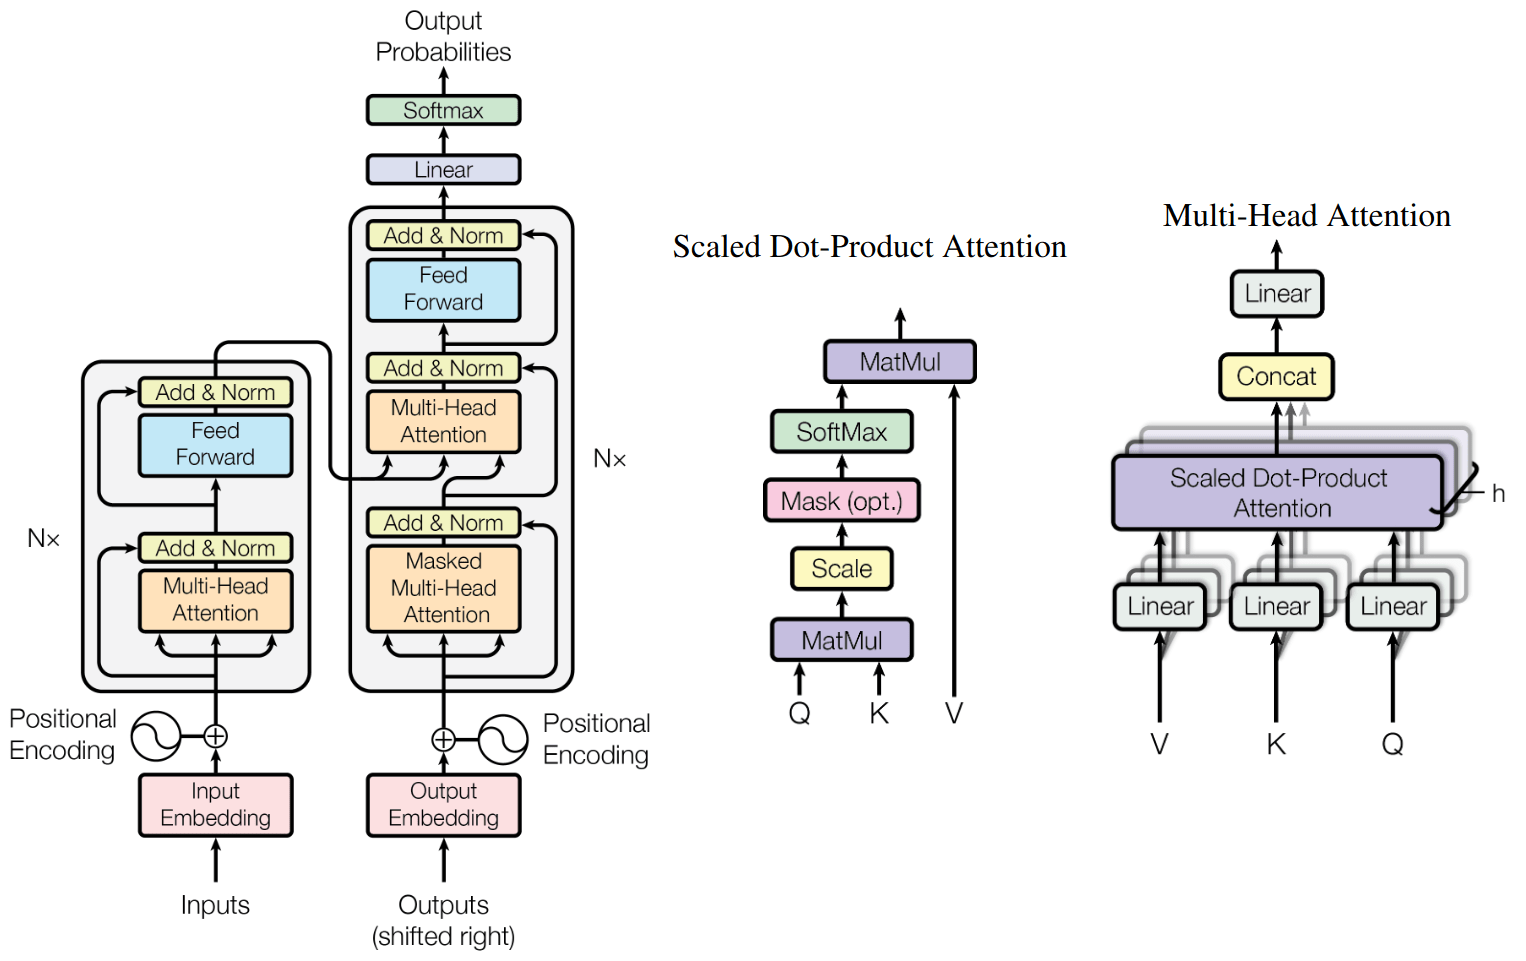
\includegraphics[width=\textwidth]{images/transformer.png}
\caption{From left to right: the Transformer architecture, the Scaled Dot-Product Attention and the Multi-Head Attention, consisting of several attention layers running in parallel \cite{attention_is_all_you_need}.}
\label{fig:transformer}
\end{figure}

The decoding part shares the same structure of the encoding part, but each decoder adds, between the self-attention and the feed-forward layer, an extra attention layer that helps the decoder focus on the important parts of the input sequence \cite{attention_is_all_you_need}.

The Transformer architecture has strong generalization capabilities, it is more efficient than sequential models since it is able to process sequential data in parallel, and it is easy to scale to large amounts of data. 

\subsubsection{Embedding} 
In a Transformer architecture, each element is mapped to a unique embedding. The purpose of embedding is to provide the model with information about what each token of the input sequence represents. Through this process the model can find over time better and better representations for the input.

Since Transformers process sequential data in parallel, they do not have a representation of the order of the inputs in the sequence. Positional encoding adds information about where each element is in the sequence; some common approaches include adding a sinusoidal function to the input sequence or to learn the encoding from scratch during training.

\subsubsection{The Attention Mechanism}
First introduced by \cite{seq2seq}, the attention mechanism allows the model to ``pay attention" to the different parts of the input sequence in order to learn which parts are more relevant for the final prediction. For each element of the input sequence, the attention mechanism computes a score that indicates its importance for the current prediction. The score is computed by taking into account the context and other relevant information from the input sequence. Elements with higher scores contribute more to the final prediction.
